\chapter{Automated Vulnerability Analysis of Smart Contracts on Ethereum} 
\label{ch:Slither-simil}

% \textit{
% This chapter is adapted from work supervised by Jeremy Clark and Mohammad Mannan, and is accepted for publication at the 2022 Workshop on Trusted Smart Contracts (WTSC) co-located with Financial Cryptography and Data Security (FC).
% }

\section{Introductory Remarks}
Smart contracts, the universal and vital programs that are deployed on blockchains, have gained increasing attention with the rapid development of blockchains.
For example, more than 10 million smart contracts have been deployed on the Ethereum Mainnet.

smart contract is an event-driven, state-based program that is written in high level languages such as Solidity.
Smart contracts have been widely used in many business domains to enable efficient and trustful transactions.

Unlike general programs, the development of smart contracts requires special effort due to their unique characteristics.
First, smart contracts are more bug intolerant compared with general programs.
“Code is law”, a smart contract can not be modified once it has been released. 
This is because transactions of a smart contract always involve cryptocurrencies which are worthy of millions of dollars (e.g. The DAO). 
A bug in a smart contract may lead to a substantial loss.
Therefore, ensuring the correctness of contracts before releasing is critical.
 This requires us to reuse experience of developed contracts in the past when developing new contracts.
Program mining for smart contracts such as summarization, checking, and code search can greatly facilitate the development and maintenance of smart contracts.
The conventional statistical analysis tools for detecting weaknesses in smart contracts purely rely on manually defined patterns, which are likely to be error-prone and can cause them to fail in complex situations.
As a result, expert attackers can easily exploit these manual checking patterns.
To minimize the risk of the attackers, machine learning powered systems provide more secure solutions relative to hard-coded static checking tools.

Throughout our research, we noticed the future direction of the literature on smart contract vulnerability detection, and our goal is to provide guidance for new developments in this field.
In order to set the ground for further development of ML method on smart contract vulnerability detection, in this survey paper, we reviewed many ML-driven intelligent detection mechanism on the following databases: Google Scholar, Engineering Village, Springer, Web of Science, Academic Search Premier, and Scholars Portal Journal.
We provided our insights on limitations and advancement of ML-driven solutions.


\section{Existing Analysis Tools}

Classic software testing technologies applied towards smart contract security analysis can be diivied into three categories; In the following, we will go over the tools proposed from the perspective of the technology they employ to tackle the smart contract security problem:

\paragraph{Static Analysis}
Static analysis is the method of analyzing a computer program of a program without running it, which can be performed at both source code and bytecode level.
Tools that employ the method of static analysis are able to scan the entirety of a code base base but also produce much false positives in the results of their scans.
SolidityCheck~\cite{soliditycheck} retrieves each function at the source code level and checks the piece that matches the pre-defined vulnerability patterns.
Normally, other tools will first obtain binary bytecode, and then use it to construct a custom intermediate representation, which have a series of forms, like SSA used in Slither~\cite{slither}, Datalog used in Securify~\cite{securify} and MadMax~\cite{madmax}, XML parsing tree used in SmartCheck~\cite{smartcheck} and XCFG used in ClairvOyance~\cite{ClairvOyance}.
Based on this representation, vulnerability pattern definition and matching are performed to screen out suspected code snippets.
As a static analysis method based on mathematical proof, formal verification is also widely used to verify the logical integrity of smart contracts, such as EtherTrust~\cite{etehrTrust}, VeriSmart~\cite{verismart} and Zeus~\cite{kalra2018zeus}.

\paragraph{Dynamic Analysis}
Fuzzing is a method of discovering software failures by constructing unexpected input data and monitoring the abnormal results of the target program during execution.
It allows developers to ensure a uniform standard of quality through prepared tests, but does not narrow down the causes of detected bugs.
When applied to smart contracts, a fuzzing engine will first try to generate initial seeds to form executable transactions.
With reference to the feedback of test results, it will dynamically adjust the generated data to explore as much smart contract state space as possible.
Finally, it will analyze the status of each transaction based on the finite state machine to detect whether there is an attackable threat.
ContractFuzzer~\cite{contractfuzzer} is the first to apply fuzz testing to smart contracts. Later, other researchers start to study improvements to different parts of fuzzing.
ReGuard~\cite{liu2018reguard} and Harvey~\cite{wustholz2020harvey} are dedicated to generating diverse inputs and transactions that are more likely to reveal vulnerabilities, ILF~\cite{he2019learning} and sFuzz~\cite{nguyen2020sfuzz} target at designing more effective generation or mutation strategy.

\paragraph{Symbolic Execution}
When using symbolic execution to analyze a program, it will use symbolic values as input instead of the specific values during the execution.
When a fork is reached, the analyzer will collect the corresponding path constraints, and then use a constraint solver to obtain specific values that can trigger each branch.
Symbolic execution can simultaneously explore multiple paths that the program can take under different inputs, but it also faces unavoidable problems such as path explosion.
In most cases, the symbolic executor will first build a control flow graph based on Ethereum bytecode, then design corresponding constraints based on the characteristics of smart contract vulnerabilities, and finally use the constraint solver to generate satisfying test cases; for example, Oyente~\cite{oyente}, Mythril~\cite{mythril}.
In recent years, there has been continuous research to optimize the process of symbolic execution.
Manticore~\cite{mossberg2019manticore} adds the support of exotic execution environments, DefectChecker~\cite{chen2021defectchecker} extracts defect related features to help improve efficiency, sCompile~\cite{chang2019scompile} identifies critical paths which involve monetary transaction and VerX~\cite{permenev2020verx} focuses on verifying effectively external callback free contracts.

\section{Deep Learning in Smart Contracts} \label{sec:dl-models}

In this section, we will go over some of the literature focusing their efforts on replacing the existing tools' capabilities explained in the previous section with amchine learning-based techniques. Afterwards, we will go over our own developed tool, \slithersimil.

There have been a lot of efforts focused towards utilizing ML based techniques in the field of vulnerability mitigation with a specific focus on the programming language Solidity and its lower level representations.

In 2018, Goswami et al. mentioned that while existing symbolic tools (e.g., Oyente) for analyzing vulnerabilities have proven to be efficient, their execution time increases significantly with depth of invocations in a smart contract ~\cite{grech2019gigahorse}.
They proposed an LSTM neural network model to detect vulnerabilities in ERC-20 smart contracts in an effort to produce a less time consuming and efficient alternative to symbolic analysis tools.
The preprocessing steps followed in this paper were very similar to the methods used by ~\cite{madmax}.
The model was trained and tested on a dataset of 165,652 ERC-20 smart contracts, which consisted of bytecode data labeled by Maian and Mythril (statistical code analysis tools).
The proposed model achieved 93.26\% accuracy, 92\% recall and an F1 score of 93\% on the testing set.
Further they have compared the time performance of their model to those of the symbolic analysis tools Maian and Mythril (static analysis tools).
While their proposed model had a runtime of 15 seconds on a testing set of 5,000 random tokens, Maian and Mythril took 32,476 and 9,475 seconds respectively.
These results indicate the same type of improvement achieved over symbolic analysis tools as in ~\cite{grech2019gigahorse}.

In 2018, Liao et al. have adopted a sequence learning approach to detect smart contract security threats ~\cite{madmax}.
Smart contract data was obtained from the Google Big Query Ethereum blockchain dataset.
Ultimately, an LSTM model was trained on 620,000 contracts from this source. Once again, the derived opcodes from the contracts were represented as one-hot vectors.
As this type of representation results in highly sparse and uninformative features, these vectors were transformed into code vectors using embedding algorithms, resulting in lower dimensionality and a higher capability of capturing potential relationship between sequences.
As another preprocessing step, they have compared the statistical properties of the opcode lengths of contracts that were identified as vulnerable and safe.
Having observed that the properties of the two categories differ significantly, they have limited the input data to the LSTM to only include contracts that had a maximum opcode length of 1600, as a design choice.
Further, the distribution of the dataset (labeled by MAIAN) was realized to be imbalanced with non-vulnerable instances making up 99.03\% of the dataset.
Therefore, all vulnerable contracts were grouped together and oversampled to achieve a balanced distribution in the training set using the Synthetic Minority Oversampling Technique (SMOTE).
The results indicated the superiority of a sequential learning approach over symbolic analysis tools.
The model achieved a vulnerability detection accuracy of 99.57\% and F1 score of 86.04\%.

In 2019, SoliAudit model was proposed to enhance the vulnerability detection of smart contracts ~\cite{etehrTrust}.
Smart contract source code in Solidity is converted into an opcode sequence to preserve the structure of executions.
Each contract goes through both a dynamic fuzzer and a vulnerability analyzer.
The vulnerability analyzer consists of a static machine learning classifier, which detects vulnerable classes, whereas the fuzzer (this term was introduced in an earlier paper) will parse the Application Binary Interface (ABI) of a smart contract to extract its declared function descriptions, data types of their arguments and their signatures.
It will then return the smart contract inputs and functions that are identified as vulnerable.
The idea of a smart contract fuzzer was introduced by the authors of ~\cite{etehrTrust}.
Vulnerability analyzer used a set of labels (13 vulnerabilities) determined by analysis tools such as Oyente and Remix.
Before training the opcode sequence data using these labels, two types of feature extraction methods were tested. These were namely, n-gram with tf-idf and word2vec.
The experiments were carried out by applying the former method together with algorithms such as Logistic Regression, Support Vector Machine, K-Nearest Neighbor, Decision Trees, Random Forests and Gradient Boosting.
The output from the latter (word2vec) was a matrix and a Convolutional Neural Network (CNN) was preferred to train it as it considers the inner structure of the matrix.
However, this combination of feature extraction and training did not yield good results.
The best results for the classification of vulnerabilities were obtained using Logistic Regression with an accuracy of 97.3\% and F1 score of 90.4\%.

In 2020, Xing et al. ~\cite{hu2021comprehensive} developed a new feature extraction method called slicing matrix, which consists of segmenting the opcode sequences derived from smart contract bytecodes to extract opcode features from each one individually.
The purpose of this segmentation is to separate useful and useless opcodes.
The extracted opcode features are then combined to form the slice matrix.
To carry out a comparative analysis, three models were created.
These were namely Neural Network Based on opcode Feature (NNBOOF), Convolution Neural Network Based on Slice Matrix (CNNBOSM), Random Forest Based on opcode Feature (RFBOOF) ~\cite{hu2021comprehensive}.
These three models were each tested on three different vulnerability classification tasks: greedy contract vulnerability, arithmetic overflow/underflow vulnerability and short address vulnerability.
While RFBOOF achieved the best results in all three cases based on precision, recall and F1 evaluation metrics, CNNBOSM performed slightly better than NNBOOF in general.
The authors mention that the slice matrix feature need further exploring.

In 2020, In N. Lesimple et al.'s paper ~\cite{day2019ethereum}, the authors study the effect of deep learning models when used to identify vulnerabilities in Smart Contracts.
It specifically highlights the vulnerabilities relating to Domain Specific Languages (DSL), which is defined as a language engineered to work solely on a single program.
This is highly relevant for blockchain, as Solidity was specifically designed for Ethereum, and therefore is a DSL.
The authors then identify some common vulnerabilities in traditional smart contract code, and examine issues with traditional vulnerability checking techniques.
Of these, one of the most important issues with traditional techniques is that the subset of bugs found are due to the strict predefined inputs that are used.
The paper proposes that, through the use of Deep Learning, the input can be varied significantly to identify faults that the predefined static tests would otherwise not.
The authors then propose a novel approach, which analysis the line level code and trains a Deep Learning Neural Network to understand the control paths and data transformations occurring in the code ~\cite{day2019ethereum}.
As an input to the model, to allow for the model to understand the code on a line level, the authors used an Abstract Syntax Tree (AST) structure, which relates variables to one another, marking their dependencies and transformations throughout the code.
The author analyzed several Natural Language Processing techniques, and Recurrent Neural Networks, and eventually landed on using an LSTM network to train their model.
They found that LSTM's outperformed most RNN models, and due to the vast variety in code syntax, the NLP techniques were unable to interpret many situations, since the code and inputs were inconsistently structured.
Their results were quite accurate, but it is important to note that the results were tested against results from a traditional model that they were actually attempting to replace.
If this paper could acquire a test set of vulnerabilities that were not acquired through the use of a traditional method, the results would be more poignant.

In 2021, Liu Z. et al. proposed a combining GNN and expert knowledge based machine learning model for detecting various smart contract vulnerabilities ~\cite{hwang2020gap}.
A graph neural network (GNN) is a deep learning method, where the principle is to perform inference on data described by graphs.
In computer science, a graph is a data structure consisting of two components: nodes (vertices) and edges. Researches have proven that written programs can be converted to symbolic graph representation, without disrupting semantic relationship between programming elements.
Thus, smart contract codes can be represented as contract graphs.
In the experiment, ESC (Ethereum Smart Contracts) and VSC (VNT chain Smart Contracts) real world datasets (containing 320,000 contracts), where ESC was used to evaluate timestamp dependence vulnerabilities, while contracts from VSC is utilized for infinite loop vulnerabilities.
The proposed model consists of two different parallel processes (Security pattern extraction and contract graph extraction) at the beginning, and the combining layer merged patterns in each section to find vulnerabilities, as shown in figure 3.
First, a feed-forward neural network generates the pattern feature for extracting security patterns from the contract's source code.
They have used an opensourced tool to extract the expert patterns from smart contract functions.
The second process (message propagation phase) is to create a GNN to achieve a contract graph.
Inside the GNN model, nodes were the program elements (i.e., function), where edges represented the flow (i.e., next function to be executed) of each program elements.
Later, unwanted nodes and edges are removed based on a node elimination strategy.
As a preprocessing method, the authors casted rich control and data flow semantics of the source code into a contract graph.
After this step, they designed a node elimination stage to highlight critical nodes by normalizing the graph.
These two parallel processes were combined using vulnerability detection phase, where both extracted features are combined convolution and full-connected layer.
In experiment, the proposed model is compared with non-ML-based security detection algorithms, namely Oyente, Myhrill, Smartcheck, Securify, and Slither.
Each algorithm and the proposed model performed a search of several vulnerabilities (re-entrancy, timestamp dependence, and infinite loop vulnerabilities) of each function in the source code.
aThe proposed algorithms (CGE) achieved 89\% accuracy on finding re-entrancy and timestamp dependence type of vulnerabilities, and 83\% accuracy on detecting infinite loop vulnerability ~\cite{hwang2020gap}.

In 2021, Eth2Vec model is proposed to deficiency in current vulnerability detection tools when a code is rewritten. In programming languages, a code rewrite is reimplementing a source code's functionality without reusing it.
When the smart contract codes are rewritten, detecting vulnerabilities become harder.
The authors first converted each smart contract source code into EVM bytecodes.
From the bytecode, the authors extracted only valuable information (i.e., function id, list of callee functions etc.) for vulnerability detection.
As the last process, a neural network structure is used to catch any vulnerabilities in the source code.
After testing the proposed model on 500 contracts, the Eth2Vec model was able to detect vulnerabilities with a 77\% precision even though the contracts are rewritten.

In 2021, O. Lutz et al.~\cite{dolan2016lava} introduce yet another method of detecting vulnerabilities within smart contracts.
The authors propose a solution entitled ESCORT, wherein they use a Deep Neural Network model to learn the semantics of the input smart contract, and learn specific vulnerability types based on the found semantics.
The goal of the ESCORT model is to overcome the scalability and generalization limitations of traditional non-DNN models.
Experimental results of this paper yielded an F1 accuracy score of 9\% on six found vulnerability types, with a detection time of 0.02 seconds per contract.
With such quick detection times, scalability is more easily achieved, satisfying one of the author's goals.
Then, through the use of transfer learning, the ESCORT model slightly overcomes the issues found in other papers, such as Y. Xu or N. Lesimple's models~\cite{grech2019gigahorse}, where newfound vulnerabilities can be realized by the model.
Unfortunately, it is rather difficult to obtain interpretability from such models, and though new vulnerabilities may be found, understanding their cause remains to be exceedingly difficult.

In 2021, Sun et al. have attempted to detect the following vulnerabilities: re-entrancy, arithmetic issues (integer overflow/underflow) and timestamp dependence using machine learning ~\cite{grech2019gigahorse}.
As a common prerequisite step, some stackoperating instructions were truncated into more general forms (e.g., SWAP1, SWAP2, ..., SWAPn. → SWAPx) to account for variations in instructions among different compilers.
Following this, opcodes were separated into 9 categories based on their functions, as a label normalization step.
As in ~\cite{etehrTrust} a word2vec transformation of the opcode sequences, preceding the convolutional layers, was performed.
In addition to the pooling and softmax layers that commonly follow convolutional layers, this paper introduces an additional self-attention layer.
The purpose of the self-attention layer is to create a connection between adjacent words in the obtained feature matrix since one-hot encoders that were used to encode each opcode instruction are just mere representatives and do not capture any functional similarity between them ~\cite{grech2019gigahorse}.
As a result, the word embedding process has been enhanced through the use of self-attention.
When compared to the vulnerability detection performance of ~\cite{etehrTrust}, they have both used a CNN but ~\cite{etehrTrust} used a word2vec embedding whereas this paper employed an attention mechanism, which is the likely reason that they obtained better results.
obtained better results. The main improvement of the created model over the existing static analyzers such as Oyente and Mythril is that it can achieve comparable performance in much less time.

In 2019, Pouyan et al. employed popular supervised ML models to classify vulnerabilities in 1000 smart contracts [7].
The dataset was built collecting 1,013 smart contracts from Etherscan, where 80\% was used for training and the remaining was used for testing purposes.
In order to label each contract based on its source code's character, they used three different feature extraction techniques: abstract syntax tree (AST), control flow graph (CFG), and Static code analysis.
The extracted features were grouped in two: features that represents execution path (e.g., function calls) and were directly added to the control flow graph. The authors used Slither and Mythrill to assign labels to each contract. 36 types of vulnerabilities were used to label each contract in test and train set. Vulnerability detection process was performed with common ML models: Support Vector Machine (SVM), Neural Network (NN), Random Forest (RF), and Decision Tree (DT). After training each model with training set, they were ranked based on the following evaluation metrics: accuracy, recall, F1, and precision. Due to the results, ML models were be able to identify 16 vulnerabilities among 36 with high performance. It was found that some specific ML models were more successful in finding certain vulnerabilities. For example, SVM model was successful of finding integer outflow, while NN achieved superior results detecting re-entrancy vulnerability. Due to the article’s summary, it was proven that extracted features of smart contracts can be passed to any popular ML model for vulnerability detection. Also, it is important to note that static code analyzers' execution time (7,311 seconds) was drastically slower than any ML model (0.32 seconds) [7]

In 2021, a vulnerability and transaction behaviour-based detection is proposed ~\cite{contractfuzzer}
 In this work, the authors built a model that correlates malicious activities, and the vulnerabilities present in smart contracts.
 In respect to strength of the correlation unsupervised ML models (K-means and HDBSCAN) assign a severity score to each smart contract.
 The model was trained to detect suspects among benign smart contracts. The aim of the research was to test their hypothesis, which was “the transaction behavior is a more critical factor in identifying malicious smart contracts than vulnerabilities in the smart contract.” Thus, they brought a different perspective to the literature of smart contracts vulnerability detection.

In 2021, Y. Xu et al.'s paper introduced two novel smart contract vulnerability detecting approach using both a KNearest Neighbors (KNN) model and a Stochastic Gradient Descent (SGD) model~\cite{slither}.
Identifying some common vulnerabilities identified by traditional methods today, they attempt to use each of the machine learning models to identify eight of the most prominently recognized traditional vulnerability types: re-entrancy, arithmetic, access control, denial of service, unchecked low level calls, bad randomness, front running, and denial of service.
As with N.Lesimple's paper~\cite{he2019learning}, the input to their model uses an AST structure, allowing the model to gather line by line information about the smart contract code.
The labels for the vulnerabilities were identified using traditional methods.
The paper notes high accuracy, precision and recall, for four of the eight vulnerabilities.
The other four did not have enough samples in the dataset, and the corresponding results were recognized as inconclusive. As with the N. Lesimple paper, the test set was created from results from using traditional methods, indicating that the authors were unable to illustrate how the KNN model differed from traditional techniques.

In 2021, ContractWard model is proposed as a faster alternative for Oyente~\cite{oyente}.
The dataset consisted of 49502 smart contracts, where each of them contained six possible vulnerabilities: integer overflow/underflow, transaction ordering dependency, call stack depth attack, timestamp dependency, and re-entrancy vulnerability.
Each contract's source code is converted to opcodes.
On average, a smart contract contains 4364 opcode elements with 100 types of opcodes in total.
After the simplification process, there were only 50 opcode types left.
Due to that reason, the authors wrapped opcodes with similar functionalities in a same category, and ultimately simplified features in the dataset.
Later, they used n-gram technique (sliding window of binary-byte size) to track relations of each opcodes, since they assume that the operations have higher relation with its neighbors.
Oyente was used to assign multi label to each contract.
After the labeling process, the researchers encountered class-imbalance problem, due to rarity of some vulnerabilities.
They employed synthetic minority oversampling technique to extend the number of minority class.
The training process adopted 5 candidate ML models: eXtreme Gradient Boosting (XGBoost), Adaptive Boosting (AdaBoost), Random Forest (RF), Support Vector Machine (SVM), and k-Nearest Neighbour (KNN).
In evolution stage, Micro-F1 and MicroF1 (variations of F1 metric) is utilized to rank the predictors.
The XGBoost model showed a robust performance by achieving over 96\% F1, Micro-F1, and Macro-F1score.

\section{\slithersimil}
Our efforts with regard to automating smart contract security assessments was to work on an addition to an already prominent static analysis tool, to better help developers and researchers in their process of auditing dmart contracts.

Trail of Bits, a prominent blockchain security firm has manually curated a wealth of data—years of security assessment reports—and we decided to explore how to use this data to make the smart contract auditing process more efficient with an addition to Slither -a static analysis tool-named Slither-simil.

Based on accumulated knowledge embedded in previous audits, we set out to detect similar vulnerable code snippets in new clients' codebases. Specifically, we explored machine learning (ML) approaches to automatically improve on the performance of Slither, our static analyzer for Solidity, and make life a bit easier for both auditors and clients.

Currently, human auditors with expert knowledge of Solidity and its security nuances scan and assess Solidity source code to discover vulnerabilities and potential threats at different granularity levels.
In our experiment, we explored how much we could automate security assessments to:
\begin{enumerate}
  \item Minimize the risk of recurring human error, i.e., the chance of overlooking known, recorded vulnerabilities.
  \item Help auditors sift through potential vulnerabilities faster and more easily while decreasing the rate of false positives.
\end{enumerate}

Slither-simil~\cite{slithersimil}, the statistical addition to Slither, is a code similarity measurement tool that uses state-of-the-art machine learning to detect similar Solidity functions.
When it began as an experiment last year under the codename crytic-pred, it was used to vectorize Solidity source code snippets and measure the similarity between them.
This year, we took it to the next level and applying it directly to vulnerable code.

Slither-simil currently uses its own representation of Solidity code, SlithIR (Slither Intermediate Representation), to encode Solidity snippets at the granularity level of functions.
We thought function-level analysis was a good place to start our research since it's not too coarse (like the file level) and not too detailed (like the statement or line level).

SlithIR is the hybrid intermediate representation used in Slither to represent Solidity code. Each node of the control flow graph can contain up to a single Solidity expression, which is converted to a set of SlithIR instructions.
This representation makes implementing analyses easier, without losing the critical semantic information contained in the Solidity source code.

SlithIR uses fewer than 40 instructions. It has no internal control flow representation and relies on Slither's control-flow graph structure (SlithIR code is associated with each node in the graph).
The complete descriptions is available at~\cite{slithir}.

\begin{figure}
  \centering
  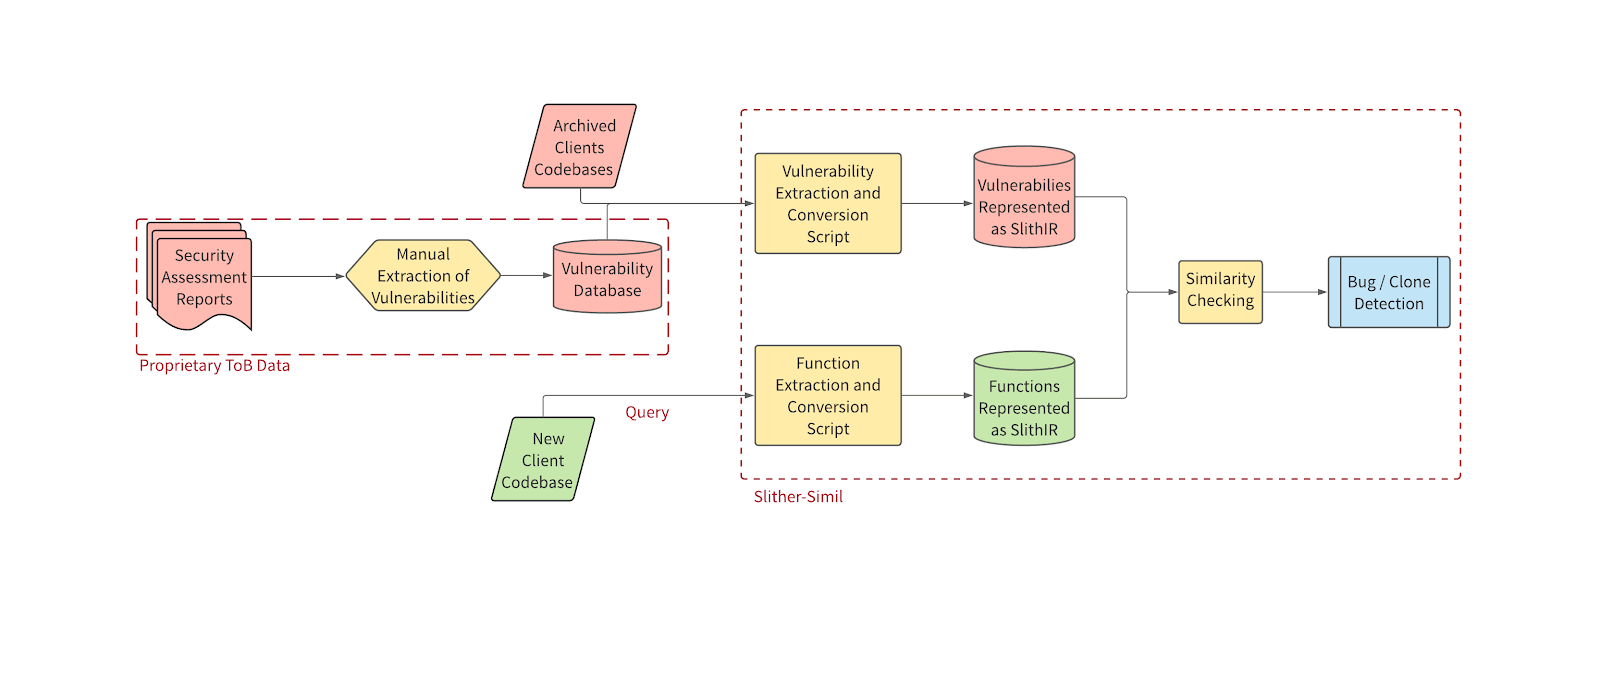
\includegraphics[width=\textwidth]{figures/slitherS.png}
  \caption{A high-level view of the process workflow of Slither-simil.}
  \label{fig:slithersimilhighlevel}
\end{figure}

In the process workflow of Slither-simil, we first manually collected vulnerabilities from the previous archived security assessments and transferred them to a vulnerability database.
Note that these are the vulnerabilities auditors had to find with no automation.

In the process workflow of Slither-simil, we first manually collected vulnerabilities from the previous archived security assessments and transferred them to a vulnerability database.
Note that these are the vulnerabilities auditors had to find with no automation.

After that, we compiled previous clients' codebases and matched the functions they contained with our vulnerability database via an automated function extraction and normalization script.
By the end of this process, our vulnerabilities were normalized SlithIR tokens as input to our ML system.

Here's how we used Slither to transform a Solidity function to the intermediate representation SlithIR, then further tokenized and normalized it to be an input to Slither-simil:

\begin{lstlisting}[float,caption= complete Solidity function from the contract TurtleToken.sol., escapechar=\%, language=Solidity, label=lst:solidity-bug]
  function transferFrom(address _from, address _to, uint256 _value) public returns (bool success) {
        require(_value <= allowance[_from][msg.sender]);     // Check allowance
        allowance[_from][msg.sender] -= _value;
        _transfer(_from, _to, _value);
        return true;
  }
  \end{lstlisting}

  \begin{lstlisting}[float,caption= The same function with its SlithIR expressions printed out., escapechar=\%, language=Solidity, label=lst:solidity-bug]
Function TurtleToken.transferFrom(address,address,uint256) (*)
 
 
Solidity Expression: require(bool)(_value <= allowance[_from][msg.sender])
SlithIR: 
         REF_10(mapping(address => uint256)) ->    allowance[_from]
         REF_11(uint256) -> REF_10[msg.sender]
         TMP_16(bool) = _value <= REF_11
         TMP_17 = SOLIDITY_CALL require(bool)(TMP_16)
 
 
Solidity Expression: allowance[_from][msg.sender] -= _value
SlithIR: 
         REF_12(mapping(address => uint256)) -> allowance[_from]
         REF_13(uint256) -> REF_12[msg.sender]
         REF_13(-> allowance) = REF_13 - _value
 
 
Solidity Expression: _transfer(_from,_to,_value)
SlithIR: 
         INTERNAL_CALL,      TurtleToken._transfer(address,address,uint256)(_from,_to,_value)
 
 
Solidity Expression: true
SlithIR: 
         RETURN True
    \end{lstlisting}


First, we converted every statement or expression into its SlithIR correspondent, then tokenized the SlithIR sub-expressions and further normalized them so more similar matches would occur despite superficial differences between the tokens of this function and the vulnerability database.

\begin{lstlisting}[float,caption= Normalized SlithIR tokens of the previous expressions., escapechar=\%, language=Solidity, label=lst:solidity-bug]
type_conversion(uint256)
 
binary(**)
 
binary(*)
 
(state_solc_variable(uint256)):=(temporary_variable(uint256))
 
index(uint256)
 
(reference(uint256)):=(state_solc_variable(uint256))
 
(state_solc_variable(string)):=(local_solc_variable(memory, string))
 
(state_solc_variable(string)):=(local_solc_variable(memory, string))
 
...
  \end{lstlisting}

After obtaining the final form of token representations for this function, we compared its structure to that of the vulnerable functions in our vulnerability database.
Due to the modularity of Slither-simil, we used various ML architectures to measure the similarity between any number of functions.

Let's take a look at the function transferFrom from the ETQuality.sol smart contract to see how its structure resembled our query function:

Comparing the statements in the two functions, we can easily see that they both contain, in the same order, a binary comparison operation (>= and <=), the same type of operand comparison, and another similar assignment operation with an internal call statement and an instance of returning a “true” value.

As the similarity score goes lower towards 0, these sorts of structural similarities are observed less often and in the other direction; the two functions become more identical, so the two functions with a similarity score of 1.0 are identical to each other.

Research on automatic vulnerability discovery in Solidity has taken off in the past two years, and tools like Vulcan and SmartEmbed, which use ML approaches to discovering vulnerabilities in smart contracts, are showing promising results.

However, all the current related approaches focus on vulnerabilities already detectable by static analyzers like Slither and Mythril, while our experiment focused on the vulnerabilities these tools were not able to identify—specifically, those undetected by Slither.

Much of the academic research of the past five years has focused on taking ML concepts (usually from the field of natural language processing) and using them in a development or code analysis context, typically referred to as code intelligence.
Based on previous, related work in this research area, we aim to bridge the semantic gap between the performance of a human auditor and an ML detection system to discover vulnerabilities, thus complementing the work of Trail of Bits human auditors with automated approaches (i.e., Machine Programming, or MP).

We still face the challenge of data scarcity concerning the scale of smart contracts available for analysis and the frequency of interesting vulnerabilities appearing in them.
We can focus on the ML model because it's sexy but it doesn't do much good for us in the case of Solidity where even the language itself is very young and we need to tread carefully in how we treat the amount of data we have at our disposal.

Archiving previous client data was a job in itself since we had to deal with the different solc versions to compile each project separately.
For someone with limited experience in that area this was a challenge, and I learned a lot along the way. (The most important takeaway of my summer internship is that if you're doing machine learning, you will not realize how major a bottleneck the data collection and cleaning phases are unless you have to do them.)

The pie chart shows how 89 vulnerabilities were distributed among the 10 client security assessments we surveyed.
We documented both the notable vulnerabilities and those that were not discoverable by Slither.

This past summer we resumed the development of Slither-simil and SlithIR with two goals in mind:

Research purposes, i.e., the development of end-to-end similarity systems lacking feature engineering.
Practical purposes, i.e., adding specificity to increase precision and recall.
We implemented the baseline text-based model with FastText to be compared with an improved model with a tangibly significant difference in results;
e.g., one not working on software complexity metrics, but focusing solely on graph-based models, as they are the most promising ones right now.

For this, we have proposed a slew of techniques to try out with the Solidity language at the highest abstraction level, namely, source code.

To develop ML models, we considered both supervised and unsupervised learning methods.
First, we developed a baseline unsupervised model based on tokenizing source code functions and embedding them in a Euclidean space
(Figure 8) to measure and quantify the distance (i.e., dissimilarity) between different tokens.
Since functions are constituted from tokens, we just added up the differences to get the (dis)similarity between any two different snippets of any size.

The diagram below shows the SlithIR tokens from a set of training Solidity data spherized in a three-dimensional Euclidean space, with similar tokens closer to each other in vector distance.
Each purple dot shows one token.

We are currently developing a proprietary database consisting of our previous clients and their publicly available vulnerable smart contracts, and references in papers and other audits.
Together they'll form one unified comprehensive database of Solidity vulnerabilities for queries, later training, and testing newer models.

We're also working on other unsupervised and supervised models, using data labeled by static analyzers like Slither and Mythril.
We're examining deep learning models that have much more expressivity we can model source code with—specifically, graph-based models, utilizing abstract syntax trees and control flow graphs.

And we're looking forward to checking out Slither-simil's performance on new audit tasks to see how
it improves our assurance team's productivity (e.g., in triaging and finding the low-hanging fruit more quickly).
We're also going to test it on Mainnet when it gets a bit more mature and automatically scalable.

You can try \slithersimil~now on Github.
For end users, it's the simplest CLI tool available:
Input one or multiple smart contract files (either directory, .zip file, or a single .sol).
Identify a pre-trained model, or separately train a model on a reasonable amount of smart contracts.

\section{Concluding Remarks}

In this chapter, we explored multiple machine learning techniques to identify vulnerabilities in smart contracts.
Amongst them, deep learning algorithms were used in a variety of ways, with different types of input
that allowed the models to identify vulnerabilities that the traditional methods
-like static analysis and dynamic fuzzing- sometimes could not.
The many reviewed uses of deep learning algorithms varied from one another by their design of the input structure,
and these through their input design, the models were able to recognize different vulnerabilities in a myriad of ways.
The reviewed methods utilizing classical machine learning methods were largely developed in a similar fashion:
to design a unique input structure for the model, to provide it with as much information relating to the structure
and purpose of the smart contract as possible.
The structure of the models themselves changed in each of the reviewed cases,
though the models accuracy and effectiveness was largely dependent on the structure of the model's input.
One of the largest benefits of this wide variety in input space, is that implementer is not dependent on a specific type of information.
For instance, if an individual cannot easily gain access to the smart contract source code, they can still utilize the transaction metadata to effectively detect vulnerabilities.
Generally, it was found that the machine learning models outperformed the traditional methods in their efficiency, and matched their effectiveness.

Throughout this review, several lackings were noticed for the existing machine learning implementations in the literature.
The first was the common labelling techniques used, which used traditional methods to label their input data.
Most of the suggested models relied on supervised models, meaning labelled data was required for the model to train.
To acquire the labels, to recognize the smart contracts as vulnerable or benign, traditional methods such as Oyente were used.
As a result, the machine learning models were attempting to recognize vulnerabilities that were already interpretable through traditional methods.
To improve this, manual detection of vulnerabilities should be implemented, or more unsupervised approaches should be explored.
A second flaw found in many of the review approaches, was the inability for the models to provide interpretability.
Due to the nature of machine learning models, sometimes the patterns found cannot be explained, and as a result, if a contract is found to be vulnerable, it becomes impossible to explain why.
This is especially true when dealing with unsupervised approaches, as the models may identify vulnerabilities in code,
but not have a defined labels to explain to any human why the contract was vulnerable.
Since interpretability is an extremely important requirement when dealing with identifying vulnerabilities,
further thought will have to be put into unsupervised approaches, to ensure the user knows why their contract is vulnerable.
In conclusion, machine learning techniques provide many newly effective ways to identify Ethereum smart contract vulnerabilities,
but more research is needed to provide solutions that outperform the traditional methods on moer vulnerabilities, with more true positives.

We also proposed \slithersimil; a powerful tool with potential to measure the similarity between function snippets of any size written in Solidity.
We are continuing to develop it, and based on current results and recent related research, we hope to see impactful real-world results before the end of the year.
But there is a lacking here and that is the bottleneck of datasets that help us train and test bigger and more comprehensive modelsl.
In the next chapter we will introduce \etherbase and how the development of \slithersimil~has extended into the development of \etherbase as a solution for us and the broader research community.